目標値変更のシミュレーションによって制御器に関する各パラメータの有効な値を探索する。 シミュレーションにはJAMOXを用いた。
% --------------------------------------------------------------------------------------
\section{重み行列の変更による制御性能評価}
	LQ最適制御に基づく状態フィードバック$F$を設計するために
	連続時間線形二次レギュレーターを用いる。この時、連続時間線形二次レギュレーターには
	システム行列$A$と入力行列$B$と重み行列$Q,R$が必要である。
	重み行列は、(\ref{eq:Feq1})式で与え、この重み行列を
	調整することで倒立振子の安定化制御の性能を高めることができる。
	そこで、シミュレーションを用いて重み行列を変更させたときの制御性能について考察していく。
	\par
	今回は行列$R$の値は変更しないので、行列$Q$のみ値を変更してシミュレーション結果を考察する。
	便宜上、重み行列$Q$の対角成分を左から第1成分、第2成分、第3成分、第4成分と呼ぶことにする。
	以下にシミュレーションを行う異なるパターンのパラメータをまとめた表とその時のシミュレーション結果を示す。
	\begin{table}[htb]
		\begin{center}
			\caption{重み行列の変更}
			\medskip
			
			\begin{tabular}{|c|c|c|c|}\hline
				\ \ & 重み行列$Q$ & オブザーバの極$P$ & サンプリング周期$\Delta[\rm{s}]$ \\ \hline\hline
				パターン1 & $Q_1$:$\rm{diag}(1E6,1E5,1,1)$ & $P_1$:$((-20,0),(-20,0))^{'}$ & $\Delta_1$:0.005 \\ \hline
				パターン2 & $Q_2$:$\rm{diag}(1E5,1E5,1,1)$ & $P_2$:$((-20,0),(-20,0))^{'}$ & $\Delta_2$:0.005 \\ \hline
				パターン3 & $Q_3$:$\rm{diag}(1E5,1E6,1,1)$ & $P_3$:$((-20,0),(-20,0))^{'}$ & $\Delta_3$:0.005 \\ \hline
			\end{tabular}
		\end{center}
		\label{table:QRF}
	\end{table}
	
	\begin{figure}[H]
		\centering
		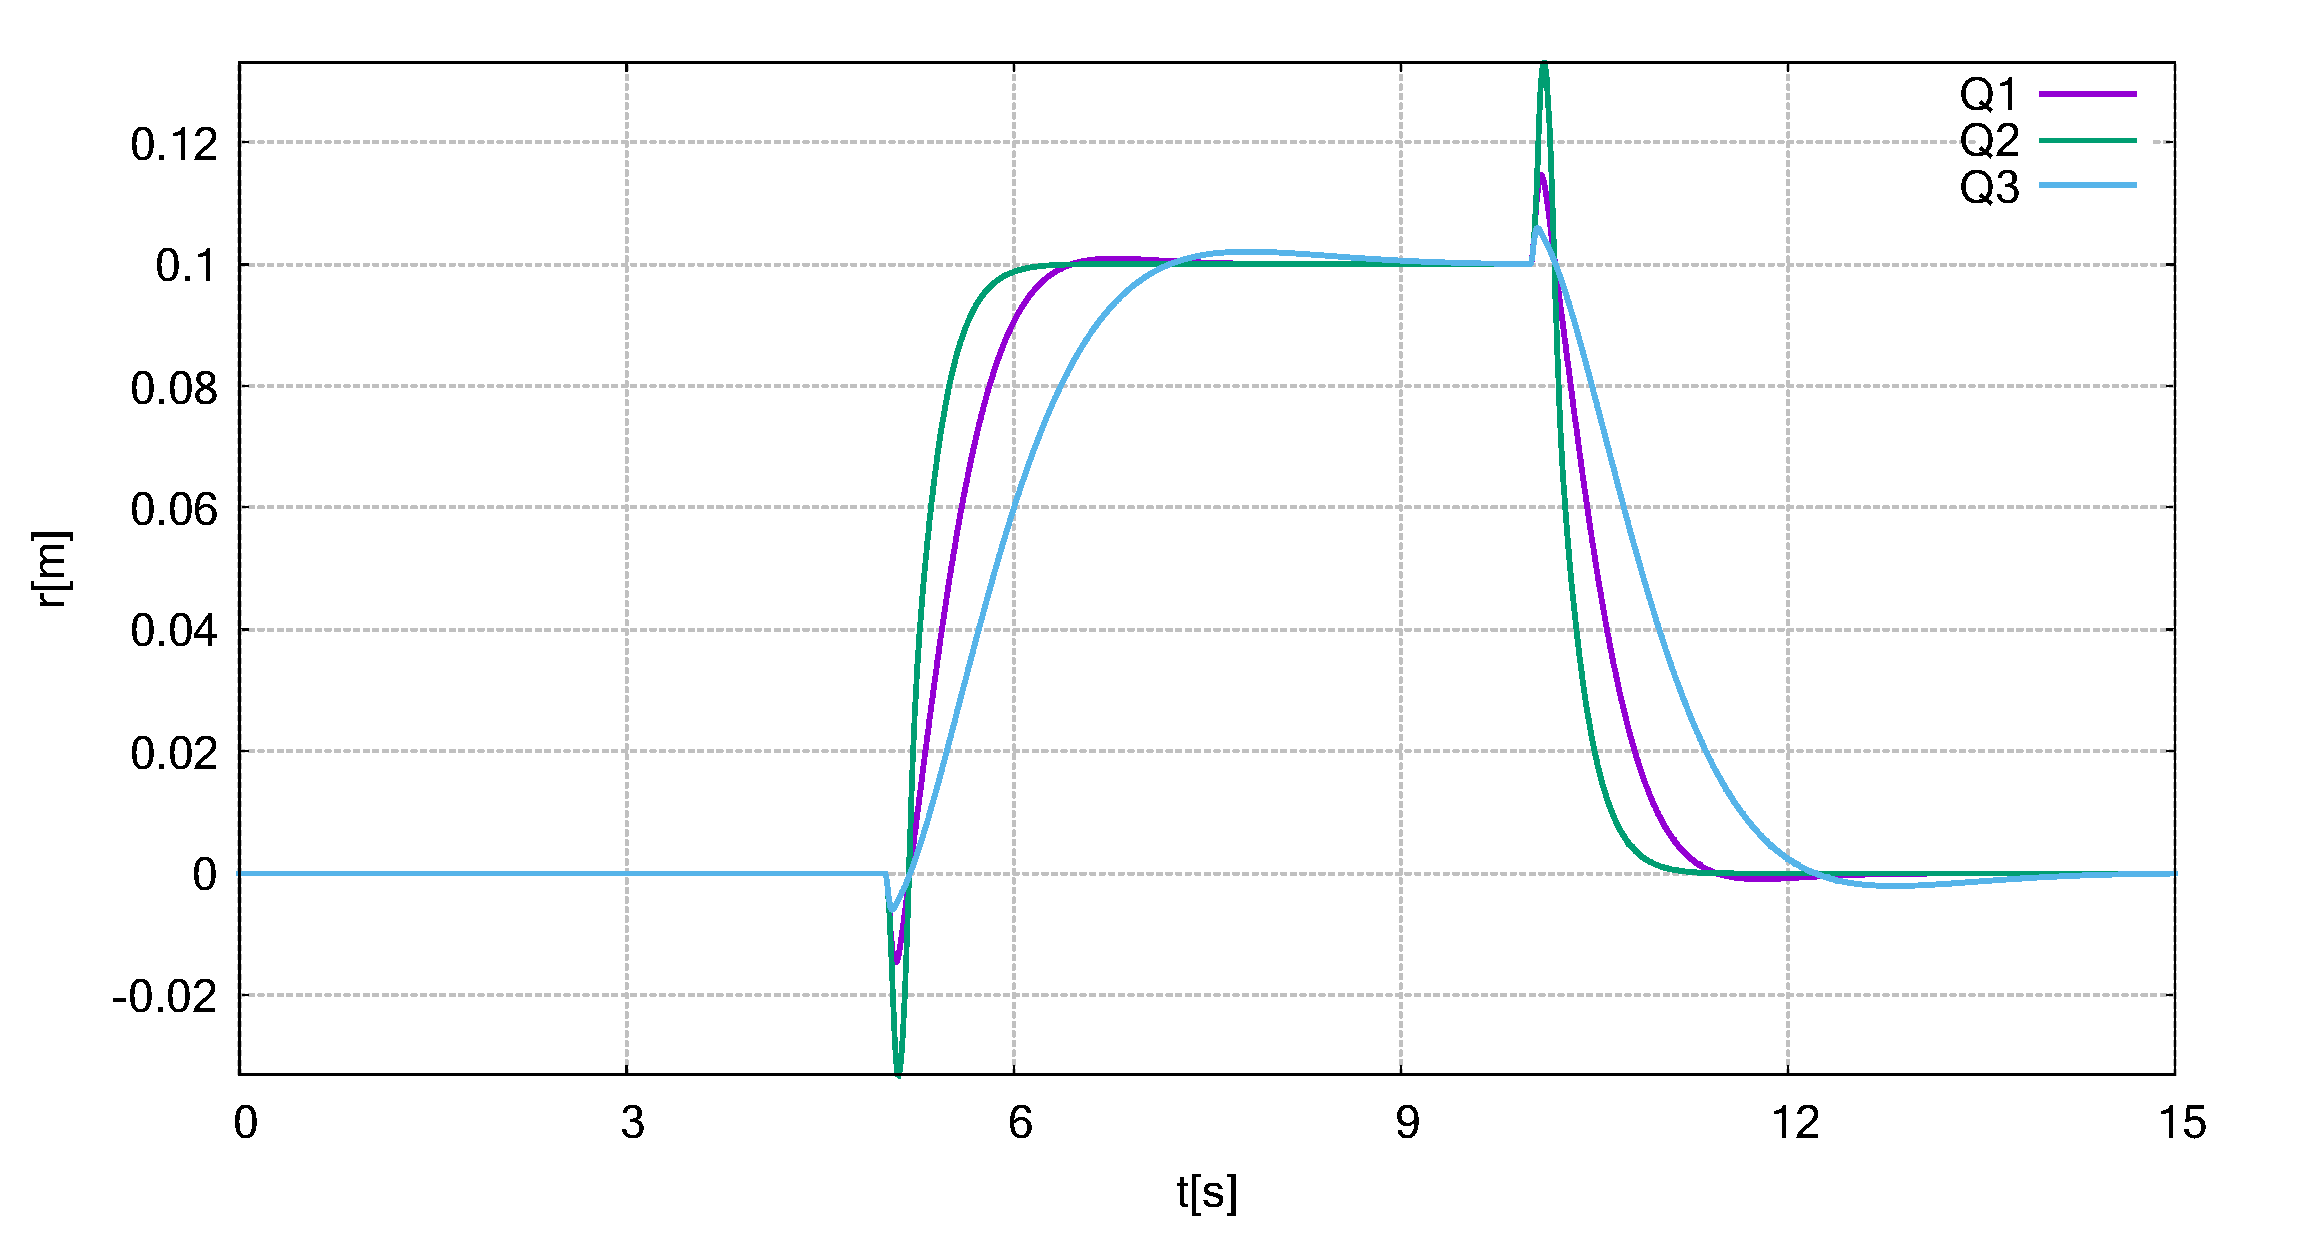
\includegraphics[width=0.8\linewidth]{gazo/simulation_QRF_compare_R.eps}
		\caption{重み行列での比較結果(台車位置)}
		\label{image:simulation_QRF_r}
	\end{figure}
	\begin{figure}[H]
		\centering
		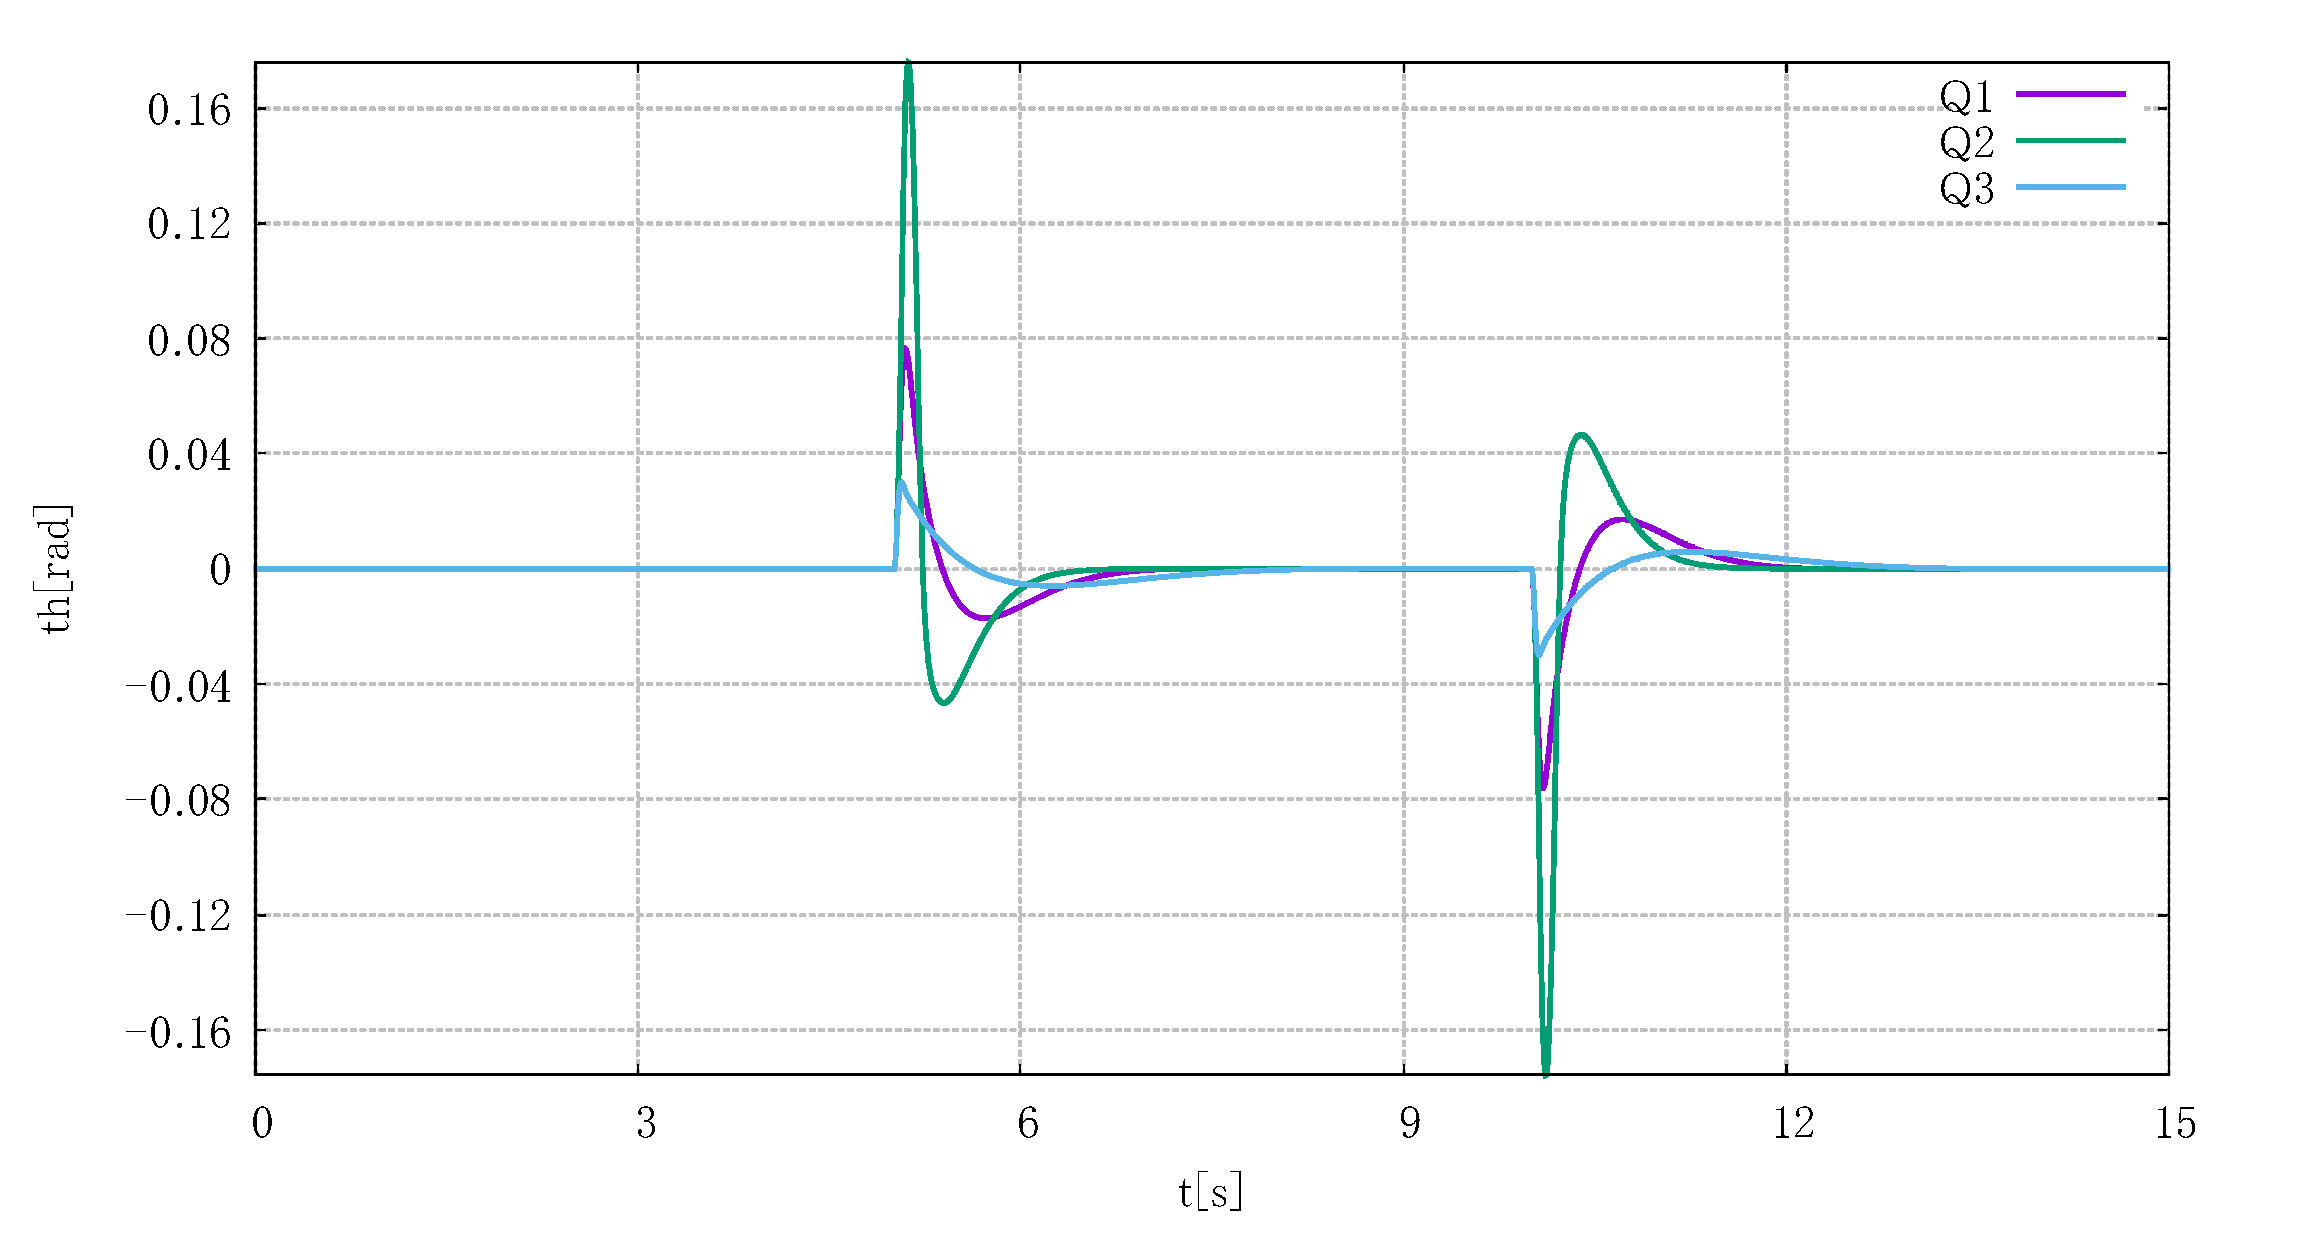
\includegraphics[width=0.8\linewidth]{gazo/simulation_QRF_compare_THETA.eps}
		\caption{重み行列での比較結果(振子角度)}
		\label{image:simulation_QRF_th}
	\end{figure}
	図(\ref{image:simulation_QRF_r})より$Q_1$の応答が一番早く、$Q_3$の応答が一番遅いことが確認できる。このことから台車の位置$r$の応答をよくするには
	重み行列$Q$の第1成分を大きくすればよいとわかる。また、$Q_1$と$Q_2$の第1成分は同じであるのにもかかわらず、$Q_2$の方が応答が早いことが確認できる。これは
	振子の角度$\theta$の応答をよくする第2成分を大きくした分、バランスが第2成分のほうに偏ってしまい、台車の位置の応答が悪くなったといえる。
	\par
	図(\ref{image:simulation_QRF_th})より、振子の角度についても同じことが言え、第2成分を大きくしている$Q_3$の応答が一番よく、$Q_1$の応答が一番悪い結果となっている。
	\par
	以上から重み行列の調整については以下のことが言える。
	\begin{itemize}
	  \item 重み行列$Q$の各成分は$r,\theta,\dot{r},\dot{\theta}$に対応している
	  \item 応答をよくしたい状態があれば、その状態に対応する成分の値を大きくすればよい
	  \item その場合、大きくした成分に対応する状態にバランスが偏る(つまり、ほかの状態の応答が悪くなる)
	\end{itemize}
	
	
% --------------------------------------------------------------------------------------
\section{オブザーバの極の変更による制御性能評価}
	前章で述べたように、最小次元オブザーバを設計するためにゴピナスの方法を用いる。
	この時、システム行列$A$、入力行列$B$、出力行列$C$、オブザーバの極$P$が必要である。
	オブザーバの極$P$を調整することで倒立振子の安定化制御の性能を高めることができる。
	同様にシミュレーションによって制御性能を考察していく。
	\par
	1つ考慮しなければならないのは、オブザーバの極と
	閉ループ系の極(つまり、$(A-BF)$の固有値)との位置関係である。
	閉ループ系の極のうち虚軸に最も近い極を$\lambda_{max}$としたとき、オブザーバーの極$P$は
	\[
		\rm{Re}(P) <5\rm{Re}(\lambda_{max})
	\]
	を満たす考慮して設定する必要がある。
	表(\ref{table:QRF})の$Q_2$を用いて設計した状態フィードバック$F$における閉ループ系の極は
	\begin{equation}
		D=\left[
		\begin{array}{c}
			-0.08\\
			-6.3+1.3i\\
			-6.3+1.3i\\
			-13\\
		\end{array}
		\right]
		\label{eq:Aeig}
	\end{equation}
	である。この中で一番虚軸に近い極は$-0.08$である。よって、少なくともオブザーバーの極$P$は$-0.4$
	より小さい値をとればよいとわかる。
	\par
	以下にシミュレーションを行う異なるパターンのパラメータをまとめた表とその時のシミュレーション結果を示す。
	\begin{table}[htb]
		\begin{center}
			\caption{重み行列の変更}
			\medskip
			
			\begin{tabular}{|c|c|c|c|}\hline
				\ \ & 重み行列$Q$ & オブザーバの極$P$ & サンプリング周期$\Delta[\rm{s}]$ \\ \hline\hline
				パターン1 & $Q_1$:$\rm{diag}(1E5,1E5,1,1)$ & $P_1$:$((-20,0),(-20,0))^{'}$ & $\Delta_1$:0.005 \\ \hline
				パターン2 & $Q_2$:$\rm{diag}(1E5,1E5,1,1)$ & $P_2$:$((-20,0),(-20,0))^{'}$ & $\Delta_2$:0.005 \\ \hline
				パターン3 & $Q_3$:$\rm{diag}(1E5,1E5,1,1)$ & $P_3$:$((-20,0),(-20,0))^{'}$ & $\Delta_3$:0.005 \\ \hline
			\end{tabular}
		\end{center}
		\label{table:QRF}
	\end{table}
	
	
%--------------------------------------------------------------------------------------
\section{サンプリング周期の変更による制御性能評価}
	離散化を行うサンプリング周期$\Delta$を調整することで倒立振子の安定化制御の性能を高めることができる。
	同様にシミュレーションによって制御性能を考察していく。
	ただし、サンプリング周期が短すぎると実験で用いる倒立振子系においてシステム全体がハングアップする恐れ
	があるため、そのような値においてはシミュレーションを行わない。
	\par
	以下にシミュレーションを行う異なるパターンのパラメータをまとめた表とその時のシミュレーション結果を示す。
	\begin{table}[htb]
		\begin{center}
			\caption{重み行列の変更}
			\medskip
			
			\begin{tabular}{|c|c|c|c|}\hline
				\ \ & 重み行列$Q$ & オブザーバの極$P$ & サンプリング周期$\Delta[\rm{s}]$ \\ \hline\hline
				パターン1 & $Q_1$:$\rm{diag}(1E5,1E5,1,1)$ & $P_1$:$((-20,0),(-20,0))^{'}$ & $\Delta_1$:0.005 \\ \hline
				パターン2 & $Q_2$:$\rm{diag}(1E5,1E5,1,1)$ & $P_2$:$((-20,0),(-20,0))^{'}$ & $\Delta_2$:0.005 \\ \hline
				パターン3 & $Q_3$:$\rm{diag}(1E5,1E5,1,1)$ & $P_3$:$((-20,0),(-20,0))^{'}$ & $\Delta_3$:0.005 \\ \hline
			\end{tabular}
		\end{center}
		\label{table:QRF}
	\end{table}
%--------------------------------------------------------------------------------------
\section{振り上げ制御及び安定化に対する制御性能評価}
	前節までにおいて、安定化制御における有効なパラメータを考察してきた。
	ここでは、振り上げ制御における有効なパラメータを考察する。
	$k,n$を調整することで振り上げ制御の制御性能を考察する。
	\par
	以下にシミュレーションを行う異なるパターンのパラメータをまとめた表とその時のシミュレーション結果を示す。
	\begin{table}[htb]
		\begin{center}
			\caption{重み行列の変更}
			\medskip
			
			\begin{tabular}{|c|c|c|c|}\hline
				\ \ & 重み行列$Q$ & オブザーバの極$P$ & サンプリング周期$\Delta[\rm{s}]$ \\ \hline\hline
				パターン1 & $Q_1$:$\rm{diag}(1E5,1E5,1,1)$ & $P_1$:$((-20,0),(-20,0))^{'}$ & $\Delta_1$:0.005 \\ \hline
				パターン2 & $Q_2$:$\rm{diag}(1E5,1E5,1,1)$ & $P_2$:$((-20,0),(-20,0))^{'}$ & $\Delta_2$:0.005 \\ \hline
				パターン3 & $Q_3$:$\rm{diag}(1E5,1E5,1,1)$ & $P_3$:$((-20,0),(-20,0))^{'}$ & $\Delta_3$:0.005 \\ \hline
			\end{tabular}
		\end{center}
		\label{table:QRF}
	\end{table}
	
%--------------------------------------------------------------------------------------